\documentclass[../main.tex]{subfiles}
\begin{document}

    \textbf{UML - Unified Modelling Language}
    \begin{itemize}
        \item rodzina \textbf{notacji} graficznych; unifikacja wielu obiektowych języków modelowania graficznego.
        \item służy do opisywania i projektowania stystemów informatycznych.
        \item nadzorowany przez organizacje OMG
        \item dwie podstawowe części:
        \begin{itemize}
            \item \textbf{Notacja} - składnia oraz elementy graficzne.
            \item \textbf{Metamodel} - semantyka oraz definicje pojęć języka i ich powiązań.
        \end{itemize}
    \end{itemize}
    \hfill \\
    \textbf{Sposoby użycia UML}:

    \begin{table}[H]
        \begin{center}
            \begin{tabular}{  p{5cm} p{5cm}  p{5cm} }
                \toprule
                \textbf{Szkic} & \textbf{Projekt} & \textbf{Język programowania}\\

                \cmidrule(r){1-1}\cmidrule(rl){2-2}\cmidrule(l){3-3}

                \begin{itemize}
                    \item użyteczny podczas tworzenia i odtwarzania,
                    \item charakter selektywny, nieformalny, dynamiczny.
                \end{itemize}
                &
                \begin{itemize}
                    \item użyteczny podczas tworzenia i odtwarzania,
                    \item powinien być kompletny i zawierać wszystkie istotne decyzje,
                    \item może dotyczyć tylko części systemu,
                    \item wymaga bardziej skomplikowanych narzędzi niż szkic.
                \end{itemize}
                &
                \begin{itemize}
                    \item diagramy tak szczegółowe, ze można generować kod automatycznie,
                    \item wymaga bardzo skomplikowanych narzędzi.
                \end{itemize}
                \\


                \bottomrule
            \end{tabular}
        \end{center}
    \end{table}


    \textbf{Aktor} - użytkownik systemu; ogólnie wszystkie role, które wchodzą w interakcje z systemem, komponenty \underline{odpowiedzialne
    za incijalizację} use casów.

    \textbf{Scenariusz przypadku użycia} - wyspecyfikowana \underline{sekwencja zdarzeń} między użytkownikiem a systemem.
    \begin{itemize}
        \item Zdefiniowane w pierwszej kolejności.
        \item Wyróżnia się jeden \textbf{główny scenariusz sukcesu}.
        \item Może zawierać warunki wstępne, gwarancje lub wyzwalacze.
        \item W agile development używa się \underline{skróconej wersji scenariusza} odpowiadającej
        na pytania: kto, co, dlaczego.
    \end{itemize}

    \textbf{Przypadek użycia} - \underline{zbiór powiązanych ze sobą scenariuszy} opisujących użycie systemu przez aktorów.
    Opisujemy je tekstowo, poprzez user stories lub diagramy.
    \begin{itemize}
        \item reprezentuje \textbf{funkcjonalne wymaganie} systemu;
        \item pewna historia; opisuje akcje systemu z punktu widzenia użytkownika;
        \item specyfikuje jeden aspekt zachowania bez wchodzenia w strukturę systemu;
        \item jest zorientowany na osiągnięcie celu użytkownika;
    \end{itemize}
    Diagramy przypadków użycia są używane do modelowania kontekstu i wymagań systemu.

    \begin{figure}[H]
        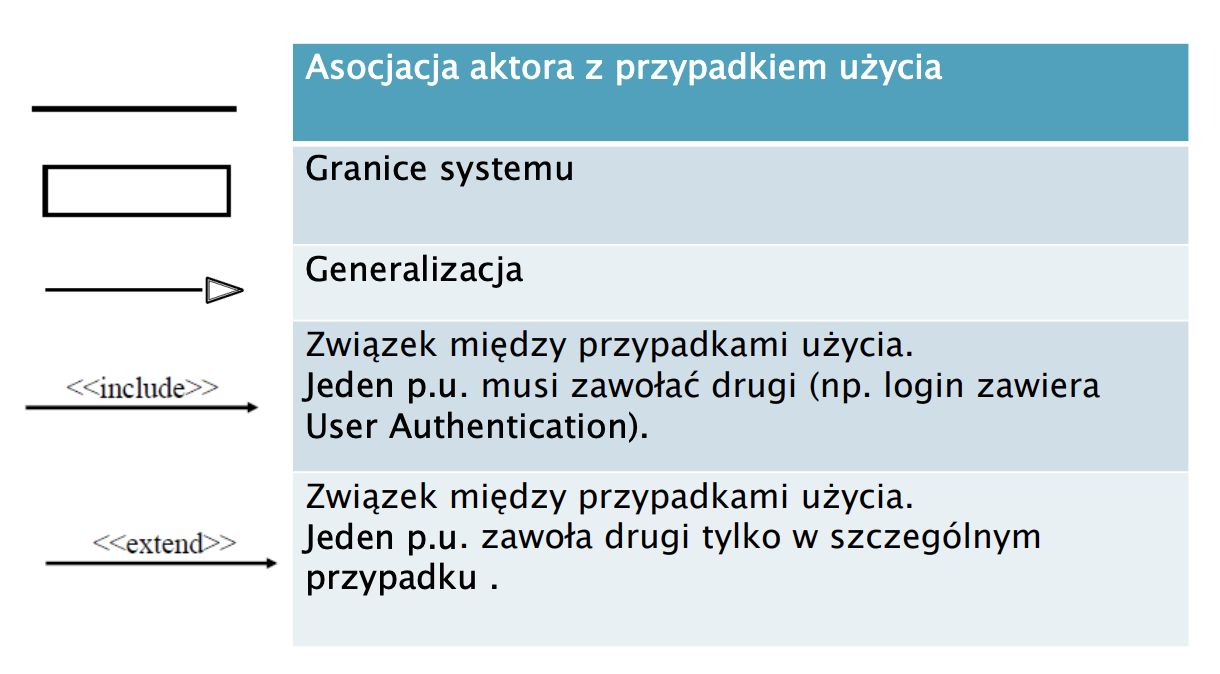
\includegraphics[width=\linewidth]{usecases.png}
    \end{figure}


    \subsection{Diagramy UML}
    \begin{table}[H]
        \begin{center}
            \begin{tabular}{  p{8cm} p{8cm} }
                \toprule
                \textbf{Strukturalne} & \textbf{Behawioralne}\\

                \cmidrule(r){1-1}\cmidrule(r){2-2}

                \begin{itemize}
                    \item diagram klas
                    \item diagram komponentów
                    \item diagram obiektów
                    \item diagram pakietów
                    \item diagram wdrożenia
                    \item diagram struktur złożonych
                \end{itemize}
                &
                \begin{itemize}
                    \item diagram czynności
                    \item diagram stanów
                    \item diagram przypadków użycia
                    \item diagram komunikacji
                    \item diagram sekwencji
                    \item diagram przeglądu
                    \item diagram przebiegów czasowych
                \end{itemize}
                \\

                \bottomrule
            \end{tabular}
        \end{center}
    \end{table}


    \subsubsection{Diagram klas}
    \begin{itemize}
        \item jeden z najczęściej używanych, zwłaszcza do \textbf{generowania kodu}.
        \item ilustracja w modelach obiektowych struktury klas i zależności między nimi,
        \item podział odpowiedzialności pomiędzy klasy i rodzaj wymienianych komunikatów,
    \end{itemize}

    \textbf{Klasy} służą do opanowania słownictwa tworzonego systemu. Używane do przedstawienia bytów programowych, sprzętowych,
    koncepcyjnych.


    \begin{table}[H]
        \begin{center}
            \begin{tabular}{ c p{8cm} }
                \raisebox{-\totalheight}{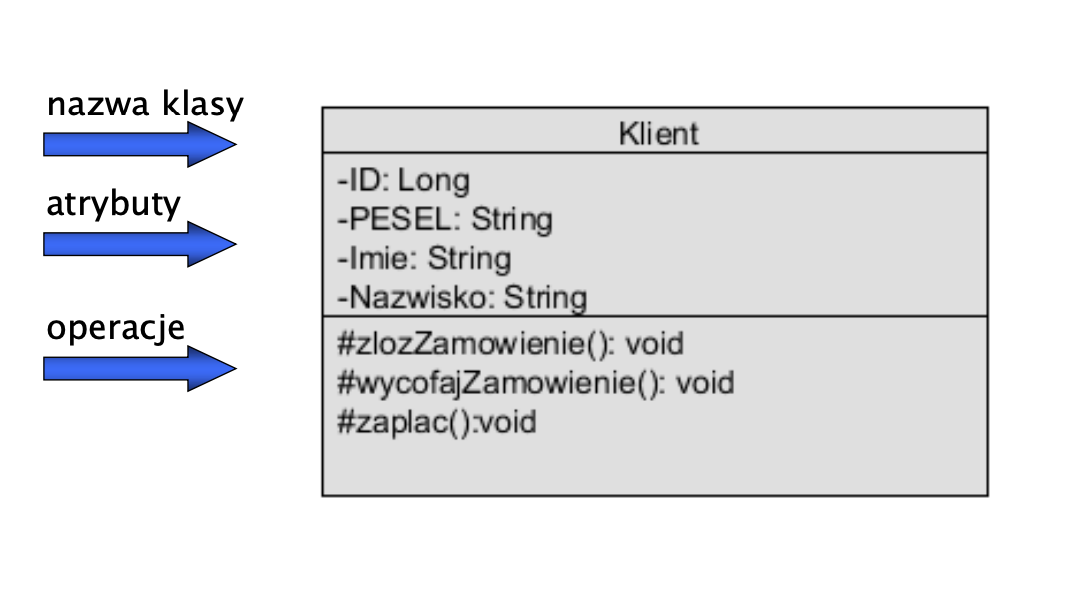
\includegraphics[width=0.5\textwidth, height=60mm]{diagram_klasy.png}}
                &
                \begin{itemize}
                    \item \textbf{Parametr} - przyjmowany przez metodę.
                    \item \textbf{Atrybut} - nazwana właściwość klasy. Może mieć podaną klasę i wartość początkową.
                    \begin{itemize}
                        \item $+$  public
                        \item \# protected
                        \item $-$ private
                    \end{itemize}
                    \item \textbf{Operacja} (metoda) - implementacja pewnej usługi, której wykonania można zarządać
                    od każdego obiektu klasy. Dokładne określenie przez podanie sygnatury (typy i domyślne wartości parametrów).
                    \item \textbf{Odpowiedzialność} - wyrażenie zobowiązań klasy (lista).

                    \item \textbf{Instancja} - każdy egzemplarz przechowuje oddzielną wartość
                    \item \textbf{Classifier} - jest tylko jedna wartość wspólna dla wszystkich egzemplarzy
                    \item \textbf{Ilość wystąpień} - liczba w prawym górnym rogu ($1 = singleton$)
                \end{itemize}
                \\
            \end{tabular}
        \end{center}
    \end{table}


    \begin{figure}[H]
        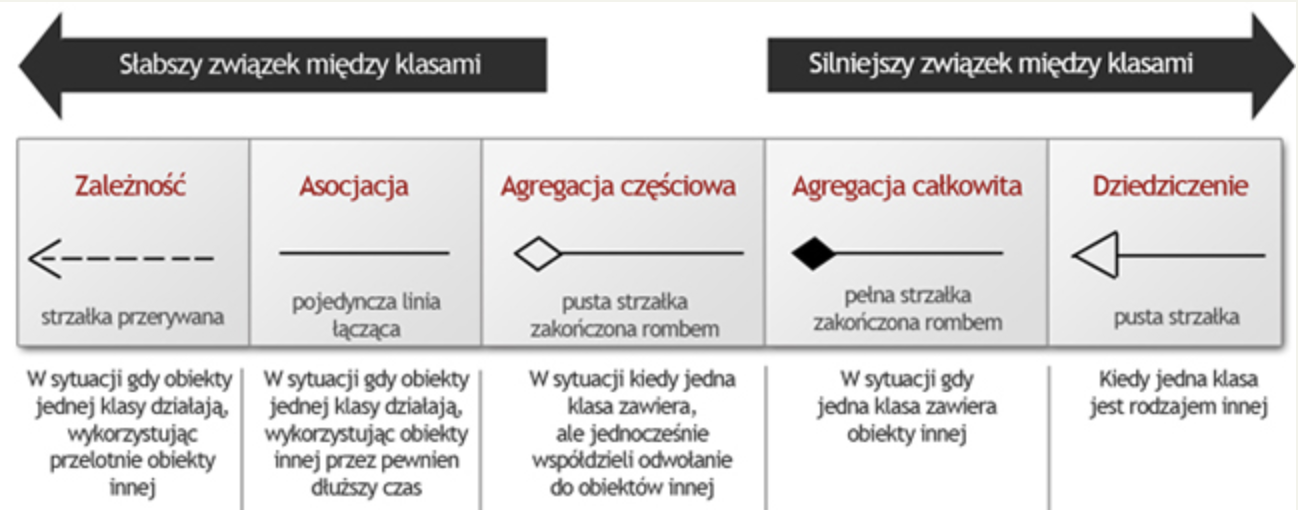
\includegraphics[width=\linewidth]{uml_zwiazki.png}
    \end{figure}

    Dodatkowo:
    \begin{itemize}
        \item \textbf{Implementacja} - linia przerywana
        zakończona pustą strzałką.
        \item \textbf{Rozszerzenia}
        \begin{itemize}
            \item \textbf{stereotypy} - służą do stworzenia nowego rodzaju obiektu ma podstawie innego obiektu
            będącego już w standardzie UML.
            \item \textbf{ograniczenia} - dotyczą zarówno klas jak i związków między nimi.
        \end{itemize}
        \item \textbf{Szablony} - klasy parametryzowane. Parametry szablony w prostokącie z przerywanych linii
        obok diagramu klasy.
    \end{itemize}



\end{document}